\subsection{Echo State Networks}

The Echo State Network is a novel approach to training RNNs in which only the
weights of the output units are adapted \cite{jaeger_echo_2001}. Fig. \ref{esn}
illustrates the basic architecture of ESN reservoirs. Applications of ESNs lie
primarily in the domain of time series prediction and classification, and the
paradigm has been successfully applied to predict myriads of benchmark time
series \cite{goudarzi_comparative_2014, alippi_quantification_2009,
rodan_minimum_2011}. Real world approaches include equalizing a wireless
communication channel \cite{jaeger_harnessing_2004}, and short-term traffic
\cite{an_short-term_2011}, electric load \cite{song_hourly_2011}, and stock
price forecasting \cite{lin_short-term_2009}.

\begin{figure}[H]
  \centering
  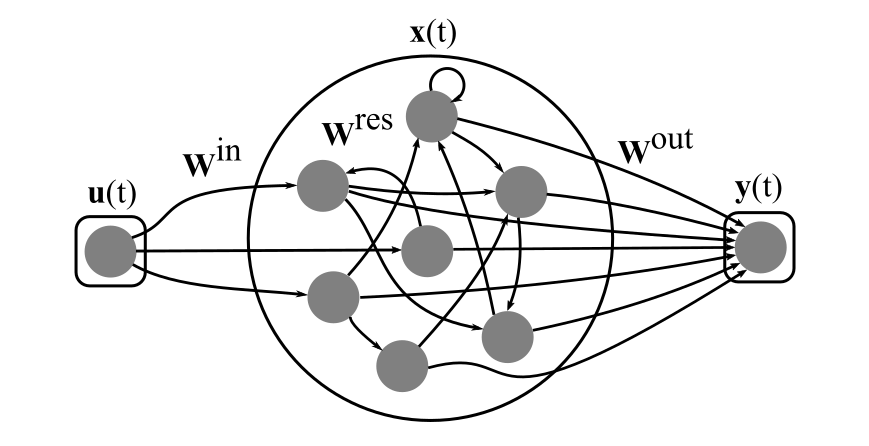
\includegraphics[width=3.0in]{img/esn.png}
  \caption{
    Basic architecture of ESN reservoir systems. The reservoir acts as a
high-dimensional kernel, transforming the temporal input sequence into a spatial
representation. The readout is trained with supervised linear regression,
providing a least squares optimum.
  }
  \label{esn}
\end{figure}

At time-step $t$, the ESN reservoir is defined by its input, internal, and
output units, denoted by $\mathbf{u}(t)$, $\mathbf{x}(t)$, and $\mathbf{y}(t)$,
respectively. The reservoir dynamics are characterized by three weight matrices,
$\mathbf{W}^{res}$, $\mathbf{W}^{in}$, and $\mathbf{W}_{out}$. In the
traditional ESN approach, the reservoir state is thus evolved according to

\begin{equation}
  \mathbf{x}(t + 1) =
    \tanh(\mathbf{W}^{res}\mathbf{x}(t)
        + \mathbf{W}^{in}\mathbf{u}(t)),
  \label{xt}
\end{equation}

\noindent using $\tanh$ as the nonlinear transfer function for internal
reservoir nodes. The output of the reservoir is given by

\begin{equation}
  \mathbf{y}(t) =
    \mathbf{W}^{out}\mathbf{x}(t).
  \label{yt}
\end{equation}

To train an ESN model of size N in a supervised and offline mode, it is run to
completion on a training set. The reservoir states are collected row-wise into a
matrix $\mathbf{X}$, and the one-dimensional output into a vector
$\mathbf{Y}$. The linear readout layer is then trained to minimize the squared
output error $E = \norm{\mathbf{Y} - \mathbf{\hat{Y}}}$ where $\mathbf{\hat{Y}}$
is the target output, which amounts to finding the $\mathbf{W}^{out}$ that
minimizes this error with linear regression. Well-known methods include ridge
regression, often called Tikhonov regularization, and the Moore-Penrose
pseudo-inverse.

When the network is adapted to $\mathbf{W}^{out}$, the ESN is fully trained,
thus illustrating the apparent simplicity and low algorithmic complexity of the
method. Gauging the performance of a trained network is done by running a test
set. We use the normalized root mean square error (NRMSE) for this evaluation,
given a predicted signal $\mathbf{y}(t)$ and a target signal
$\mathbf{\hat{y}}(t)$

\begin{equation}
  \textrm{NRMSE}(\mathbf{y}, \mathbf{\hat{y}}) = \sqrt{\frac{
      \mean{\norm{\mathbf{y}(t) - \mathbf{\hat{y}}(t)}^{2}}
    }{
      \mean{\norm{\mathbf{\hat{y}}(t) - \mean{\mathbf{\hat{y}}(t)}}^{2}}
    }
  }
  .
  \label{nrmse}
\end{equation}

As with practically every machine learning technique, the application of ESNs
requires some experience. Although a conceptually simple idea, generating
adequate reservoir networks is influenced by multiple global parameters. The
most important parameters include the scaling of the input weight matrix
$\iota$, the spectral radius of the reservoir connection matrix $\rho$, and the
model size parameter $N$ \cite{montavon_practical_2012, jaeger_tutorial_nodate}.

\subsection{Assessing the quality of a reservoir}

In the RC methodology, computation and memory retainment are intertwined, in
stark contrast to traditional architectures which use separate memory storage
units. Attributing task-solving performance to either memory capacity or
computation is therefore quite difficult.

Attempts have been made to unify quality metrics for reservoir substrates,
e.g. the ability to separate different inputs \cite{legenstein_edge_2007}, the
ability to generalize \cite{legenstein_edge_2007}, and linear short-term memory
\cite{jaeger_short_2002}.

\subsection{NARMA}

Nonlinear autoregressive moving average (NARMA) is a class of time series models
widely used to benchmark the performance of RC models \cite{atiya_new_2000,
kubota_dynamical_2019}. We have chosen the NARMA10 time series to be the main
evaluation criteria for network performance, which is a temporal task with a
time-lag of ten time steps, given by

\begin{equation}
  y_{t+1} = \alpha y_{t} +
  \beta y_{t} \sum_{i=0}^{9}y_{t-i} +
  \gamma u_{t}u_{t-9} +
  \delta,
  \label{narma}
\end{equation}

\noindent with the default constant parameters $\alpha = 0.3$, $\beta = 0.05$,
$\gamma = 1.5$ and $\delta = 0.1$. The input $u_{t}$ is an i.i.d. stream drawn
from the interval [0, 0.5]. The task is well-suited for evaluating memory
capacity and computational power with a single metric, as it presents a
challenge of both memory and nonlinearity, uncovered to be a universal trade-off
in in dynamical systems used in reservoir settings
\cite{dambre_information_2012, verstraeten_memory_2010}.

Evaluation of ESN performance on the NARMA10 system is a thoroughly explored
area in the field of RC, with the best NRMSE performances reported for
traditional ESN reservoirs of size $N = 200$ lying in the range [0.20, 0.25]
\cite{goudarzi_comparative_2014, rodan_minimum_2011,
verstraeten_experimental_2007, jaeger_adaptive_nodate}. For some context, using
a shift register containing the input as a reservoir will achieve a minimal
NRMSE of 0.4. To achieve NRMSE values below this threshold it is necessary to
introduce nonlinearity in the reservoir.

%%% Local Variables:
%%% mode: latex
%%% TeX-master: "../main"
%%% End:
